\chapter{Combinatória}

\index{combinatória}

A \key{combinatória} estuda métodos para contar
combinações de objetos.
Normalmente, o objetivo é encontrar uma maneira de
contar as combinações de forma eficiente,
sem gerar cada combinação separadamente.

Como exemplo, considere o problema
de contar o número de maneiras de
representar um inteiro $n$ como uma soma de inteiros positivos.
Por exemplo, existem 8 representações
para $4$:
\begin{multicols}{2}
\begin{itemize}
\item $1+1+1+1$
\item $1+1+2$
\item $1+2+1$
\item $2+1+1$
\item $2+2$
\item $3+1$
\item $1+3$
\item $4$
\end{itemize}
\end{multicols}

Um problema combinatório pode frequentemente ser resolvido
usando uma função recursiva.
Nesse problema, podemos definir uma função $f(n)$
que fornece o número de representações para $n$.
Por exemplo, $f(4)=8$, de acordo com o exemplo acima.
Os valores da função
podem ser calculados recursivamente da seguinte forma:
\begin{equation*}
    f(n) = \begin{cases}
               1               & n = 0\\
               f(0)+f(1)+\cdots+f(n-1) & n > 0\\
           \end{cases}
\end{equation*}
O caso base é $f(0)=1$,
porque a soma vazia representa o número 0.
Então, se $n>0$, consideramos todas as maneiras de
escolher o primeiro número da soma.
Se o primeiro número for $k$,
existem $f(n-k)$ representações
para a parte restante da soma.
Assim, calculamos a soma de todos os valores
da forma $f(n-k)$, onde $k<n$.

Os primeiros valores para a função são:
\[
\begin{array}{lcl}
f(0) & = & 1 \\
f(1) & = & 1 \\
f(2) & = & 2 \\
f(3) & = & 4 \\
f(4) & = & 8 \\
\end{array}
\]

Às vezes, uma fórmula recursiva pode ser substituída
por uma fórmula fechada.
Nesse problema,
\[
f(n)=2^{n-1},
\]
que se baseia no fato de que existem $n-1$
possíveis posições para os sinais de +- na soma,
e podemos escolher qualquer subconjunto deles.

\section{Coeficientes Binomiais}

\index{coeficiente binomial}

O \key{coeficiente binomial} ${n \choose k}$
é igual ao número de maneiras pelas quais podemos escolher um subconjunto 
de $k$ elementos de um conjunto de $n$ elementos.
Por exemplo, ${5 \choose 3}=10$,
porque o conjunto $\{1,2,3,4,5\}$
possui 10 subconjuntos de 3 elementos: 
\[ \{1,2,3\}, \{1,2,4\}, \{1,2,5\}, \{1,3,4\}, \{1,3,5\}, 
\{1,4,5\}, \{2,3,4\}, \{2,3,5\}, \{2,4,5\}, \{3,4,5\} \]

\subsubsection{Fórmula 1}

Os coeficientes binomiais podem ser
calculados recursivamente da seguinte forma:

\[
{n \choose k}  =  {n-1 \choose k-1} + {n-1 \choose k}
\]

A ideia é fixar um elemento $x$ no conjunto.
Se $x$ está incluído no subconjunto,
temos que escolher $k-1$
elementos de $n-1$ elementos,
e, se $x$ não estiver incluído no subconjunto,
temos que escolher $k$ elementos de $n-1$ elementos.

Os casos base para a recursão são
\[
{n \choose 0}  =  {n \choose n} = 1,
\]
porque há sempre exatamente
uma maneira de construir um subconjunto vazio
e um subconjunto que contém todos os elementos.

\subsubsection{Fórmula 2}

Outra maneira de calcular os coeficientes binomiais é a seguinte:
\[
{n \choose k}  =  \frac{n!}{k!(n-k)!}.
\]

Existem $n!$ permutações de $n$ elementos.
Percorremos todas as permutações e sempre
incluímos os primeiros $k$ elementos da permutação
no subconjunto.
Como a ordem dos elementos dentro e fora do subconjunto
não importa,
o resultado é dividido por $k!$ e $(n-k)!$

\subsubsection{Propriedades}

Para coeficientes binomiais,
\[
{n \choose k}  =  {n \choose n-k},
\]
porque, na verdade, dividimos um conjunto de $n$ elementos em
dois subconjuntos: o primeiro contém $k$ elementos,
e o segundo contém $n-k$ elementos.

A soma dos coeficientes binomiais é:
\[
{n \choose 0}+{n \choose 1}+{n \choose 2}+\ldots+{n \choose n}=2^n.
\]

A razão para o nome "coeficiente binomial"
pode ser vista quando o binômio $(a+b)$ é elevado à
$n$-ésima potência:

\[ (a+b)^n =
{n \choose 0} a^n b^0 + 
{n \choose 1} a^{n-1} b^1 +
\ldots + 
{n \choose n-1} a^1 b^{n-1} +
{n \choose n} a^0 b^n. \]

\index{Triângulo de Pascal}

Os coeficientes binomiais também aparecem no
\key{Triângulo de Pascal},
onde cada valor é igual à soma dos dois
valores acima:
\begin{center}
\begin{tikzpicture}{0.9}
\node at (0,0) {1};
\node at (-0.5,-0.5) {1};
\node at (0.5,-0.5) {1};
\node at (-1,-1) {1};
\node at (0,-1) {2};
\node at (1,-1) {1};
\node at (-1.5,-1.5) {1};
\node at (-0.5,-1.5) {3};
\node at (0.5,-1.5) {3};
\node at (1.5,-1.5) {1};
\node at (-2,-2) {1};
\node at (-1,-2) {4};
\node at (0,-2) {6};
\node at (1,-2) {4};
\node at (2,-2) {1};
\node at (-2,-2.5) {$\ldots$};
\node at (-1,-2.5) {$\ldots$};
\node at (0,-2.5) {$\ldots$};
\node at (1,-2.5) {$\ldots$};
\node at (2,-2.5) {$\ldots$};
\end{tikzpicture}
\end{center}

\subsubsection{Caixas e Bolas}

"Caixas e bolas" é um modelo útil,
no qual contamos as maneiras de
colocar $k$ bolas em $n$ caixas.
Vamos considerar três cenários:

\textit{Cenário 1}: Cada caixa pode conter
no máximo uma bola.
Por exemplo, quando $n=5$ e $k=2$,
existem 10 soluções:

\begin{center}
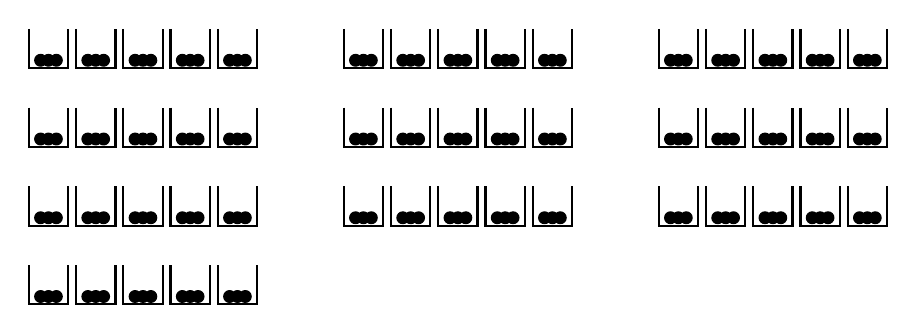
\begin{tikzpicture}[scale=0.5]
\newcommand\lax[3]{
\path[draw,thick,-] (#1-0.5,#2+0.5) -- (#1-0.5,#2-0.5) --
                    (#1+0.5,#2-0.5) -- (#1+0.5,#2+0.5);
\ifthenelse{\equal{#3}{1}}{\draw[fill=black] (#1,#2-0.3) circle (0.15);}{}
\ifthenelse{\equal{#3}{2}}{\draw[fill=black] (#1-0.2,#2-0.3) circle (0.15);}{}
\ifthenelse{\equal{#3}{2}}{\draw[fill=black] (#1+0.2,#2-0.3) circle (0.15);}{}
}
\newcommand\laa[7]{
    \lax{#1}{#2}{#3}
    \lax{#1+1.2}{#2}{#4}
    \lax{#1+2.4}{#2}{#5}
    \lax{#1+3.6}{#2}{#6}
    \lax{#1+4.8}{#2}{#7}
}

\laa{0}{0}{1}{1}{0}{0}{0}
\laa{0}{-2}{1}{0}{1}{0}{0}
\laa{0}{-4}{1}{0}{0}{1}{0}
\laa{0}{-6}{1}{0}{0}{0}{1}
\laa{8}{0}{0}{1}{1}{0}{0}
\laa{8}{-2}{0}{1}{0}{1}{0}
\laa{8}{-4}{0}{1}{0}{0}{1}
\laa{16}{0}{0}{0}{1}{1}{0}
\laa{16}{-2}{0}{0}{1}{0}{1}
\laa{16}{-4}{0}{0}{0}{1}{1}

\end{tikzpicture}
\end{center}

Neste cenário, a resposta é diretamente o
coeficiente binomial ${n \choose k}$.

\textit{Cenário 2}: Uma caixa pode conter várias bolas.
Por exemplo, quando $n=5$ e $k=2$,
existem 15 soluções:

\begin{center}
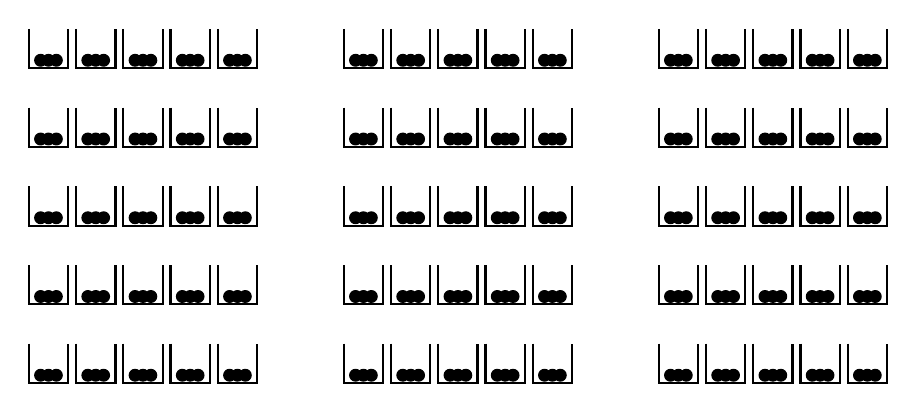
\begin{tikzpicture}[scale=0.5]
\newcommand\lax[3]{
\path[draw,thick,-] (#1-0.5,#2+0.5) -- (#1-0.5,#2-0.5) --
                    (#1+0.5,#2-0.5) -- (#1+0.5,#2+0.5);
\ifthenelse{\equal{#3}{1}}{\draw[fill=black] (#1,#2-0.3) circle (0.15);}{}
\ifthenelse{\equal{#3}{2}}{\draw[fill=black] (#1-0.2,#2-0.3) circle (0.15);}{}
\ifthenelse{\equal{#3}{2}}{\draw[fill=black] (#1+0.2,#2-0.3) circle (0.15);}{}
}
\newcommand\laa[7]{
    \lax{#1}{#2}{#3}
    \lax{#1+1.2}{#2}{#4}
    \lax{#1+2.4}{#2}{#5}
    \lax{#1+3.6}{#2}{#6}
    \lax{#1+4.8}{#2}{#7}
}

\laa{0}{0}{2}{0}{0}{0}{0}
\laa{0}{-2}{1}{1}{0}{0}{0}
\laa{0}{-4}{1}{0}{1}{0}{0}
\laa{0}{-6}{1}{0}{0}{1}{0}
\laa{0}{-8}{1}{0}{0}{0}{1}
\laa{8}{0}{0}{2}{0}{0}{0}
\laa{8}{-2}{0}{1}{1}{0}{0}
\laa{8}{-4}{0}{1}{0}{1}{0}
\laa{8}{-6}{0}{1}{0}{0}{1}
\laa{8}{-8}{0}{0}{2}{0}{0}
\laa{16}{0}{0}{0}{1}{1}{0}
\laa{16}{-2}{0}{0}{1}{0}{1}
\laa{16}{-4}{0}{0}{0}{2}{0}
\laa{16}{-6}{0}{0}{0}{1}{1}
\laa{16}{-8}{0}{0}{0}{0}{2}

\end{tikzpicture}
\end{center}

O processo de colocação das bolas nas caixas
pode ser representado como uma string
que consiste nos símbolos
"o" e "$\rightarrow$".
Inicialmente, suponha que estamos na caixa mais à esquerda.
O símbolo "o" significa que colocamos uma bola
na caixa atual, e o símbolo
"$\rightarrow$" significa que nos movemos para
a próxima caixa à direita.

Usando essa notação, cada solução é uma string
que contém $k$ vezes o símbolo "o" e
$n-1$ vezes o símbolo "$\rightarrow$".
Por exemplo, a solução superior direita
na figura acima corresponde à string
"$\rightarrow$ $\rightarrow$ o $\rightarrow$ o $\rightarrow$".
Assim, o número de soluções é
${k+n-1 \choose k}$.

\textit{Cenário 3}: Cada caixa pode conter, no máximo, uma bola,
e, além disso, duas caixas adjacentes não podem conter uma bola ao mesmo tempo.
Por exemplo, quando $n=5$ e $k=2$,
existem 6 soluções:


\begin{center}
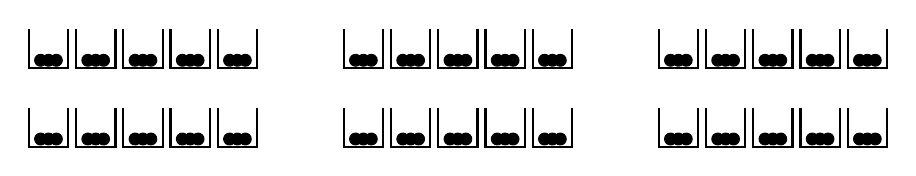
\begin{tikzpicture}[scale=0.5]
\newcommand\lax[3]{
\path[draw,thick,-] (#1-0.5,#2+0.5) -- (#1-0.5,#2-0.5) --
                    (#1+0.5,#2-0.5) -- (#1+0.5,#2+0.5);
\ifthenelse{\equal{#3}{1}}{\draw[fill=black] (#1,#2-0.3) circle (0.15);}{}
\ifthenelse{\equal{#3}{2}}{\draw[fill=black] (#1-0.2,#2-0.3) circle (0.15);}{}
\ifthenelse{\equal{#3}{2}}{\draw[fill=black] (#1+0.2,#2-0.3) circle (0.15);}{}
}
\newcommand\laa[7]{
    \lax{#1}{#2}{#3}
    \lax{#1+1.2}{#2}{#4}
    \lax{#1+2.4}{#2}{#5}
    \lax{#1+3.6}{#2}{#6}
    \lax{#1+4.8}{#2}{#7}
}

\laa{0}{0}{1}{0}{1}{0}{0}
\laa{0}{-2}{1}{0}{0}{1}{0}
\laa{8}{0}{1}{0}{0}{0}{1}
\laa{8}{-2}{0}{1}{0}{1}{0}
\laa{16}{0}{0}{1}{0}{0}{1}
\laa{16}{-2}{0}{0}{1}{0}{1}
\end{tikzpicture}
\end{center}

Neste cenário, podemos supor que
$k$ bolas são inicialmente colocadas em caixas,
e há uma caixa vazia entre cada
duas caixas adjacentes.
A tarefa restante é escolher as
posições para as caixas vazias restantes.
Existem $n-2k+1$ caixas desse tipo e
$k+1$ posições para elas.
Assim, usando a fórmula do cenário 2,
o número de soluções é
${n-k+1 \choose n-2k+1}$.

\subsubsection{Coeficientes multinomiais}

\index{coeficiente multinomial}

O \key{coeficiente multinomial}
\[ {n \choose k_1,k_2,\ldots,k_m} = \frac{n!}{k_1! k_2! \cdots k_m!}, \]
é igual ao número de maneiras
pelas quais podemos dividir $n$ elementos em subconjuntos
de tamanhos $k_1,k_2,\ldots,k_m$,
onde $k_1+k_2+\cdots+k_m=n$.
Os coeficientes multinomiais podem ser vistos como uma
generalização dos coeficientes binomiais;
se $m=2$, a fórmula acima
corresponde à fórmula do coeficiente binomial.

\section{Números de Catalan}

\index{número de Catalan}

O \key{número de Catalan}
%\footnote{E. C. Catalan (1814--1894) foi um matemático belga.}
$C_n$ é igual ao
número de expressões válidas com parênteses que consistem em
$n$ parênteses esquerdos e $n$ parênteses direitos.

Por exemplo, $C_3=5$, pois
podemos construir as seguintes expressões com parênteses usando três
parênteses esquerdos e direitos:

\begin{itemize}[noitemsep]
\item \texttt{()()()}
\item \texttt{(())()}
\item \texttt{()(())}
\item \texttt{((()))}
\item \texttt{(()())}
\end{itemize}

\subsubsection{Expressões com parênteses}

\index{expressão com parênteses}

O que é exatamente uma \emph{expressão válida com parênteses}?
As seguintes regras definem precisamente todas
as expressões válidas com parênteses:

\begin{itemize}
\item Uma expressão com parênteses vazia é válida.
\item Se uma expressão $A$ é válida,
então a expressão
\texttt{(}$A$\texttt{)} também é válida.
\item Se as expressões $A$ e $B$ são válidas,
então a expressão $AB$ também é válida.
\end{itemize}


Outra forma de caracterizar as expressões válidas
com parênteses é que, se
escolhermos qualquer prefixo de tal expressão,
ele deve conter pelo menos tantos parênteses esquerdos
quanto parênteses direitos.
Além disso, a expressão completa deve
conter um número igual de parênteses esquerdos e direitos.

\subsubsection{Fórmula 1}

Os números de Catalan podem ser calculados usando a fórmula
\[ C_n = \sum_{i=0}^{n-1} C_{i} C_{n-i-1}.\]

A soma percorre as maneiras de dividir a
expressão em duas partes,
de modo que ambas as partes sejam expressões válidas,
e a primeira parte seja a mais curta possível,
mas não vazia.
Para qualquer $i$, a primeira parte contém $i+1$ pares
de parênteses, e o número de expressões
é o produto dos seguintes valores:

\begin{itemize}
\item $C_{i}$: o número de maneiras de construir uma expressão
usando os parênteses da primeira parte,
sem contar os parênteses mais externos
\item $C_{n-i-1}$: o número de maneiras de construir uma
expressão usando os parênteses da segunda parte
\end{itemize}

O caso base é $C_0=1$,
porque podemos construir uma expressão com parênteses vazia
usando zero pares de parênteses.

\subsubsection{Fórmula 2}

Os números de Catalan também podem ser calculados
usando coeficientes binomiais:
\[ C_n = \frac{1}{n+1} {2n \choose n}\]
A fórmula pode ser explicada da seguinte forma:

Há um total de ${2n \choose n}$ maneiras
de construir uma expressão com parênteses (não necessariamente válida)
que contém $n$ parênteses esquerdos
e $n$ parênteses direitos.
Vamos calcular o número de tais
expressões que \emph{não} são válidas.

Se uma expressão com parênteses não é válida,
ela deve conter um prefixo no qual o
número de parênteses direitos excede o
número de parênteses esquerdos.
A ideia é inverter cada parêntese
que pertence a tal prefixo.
Por exemplo, a expressão
\texttt{())()(} contém um prefixo \texttt{())},
e, depois de inverter o prefixo,
a expressão se torna \texttt{)((()(}.

A expressão resultante consiste em $n+1$
parênteses esquerdos e $n-1$ parênteses direitos.
O número de tais expressões é ${2n \choose n+1}$,
que é igual ao número de expressões
com parênteses não válidas.
Assim, o número de expressões
com parênteses válidas pode ser calculado usando a fórmula
\[{2n \choose n}-{2n \choose n+1} = {2n \choose n} - \frac{n}{n+1} {2n \choose n} = \frac{1}{n+1} {2n \choose n}.\]

\subsubsection{Contando árvores}

Os números de Catalan também estão relacionados a árvores:

\begin{itemize}
\item Existem $C_n$ árvores binárias de $n$ vértices.
\item Existem $C_{n-1}$ árvores enraizadas de $n$ vértices.
\end{itemize}
\noindent
Por exemplo, para $C_3=5$, as árvores binárias são

\begin{center}
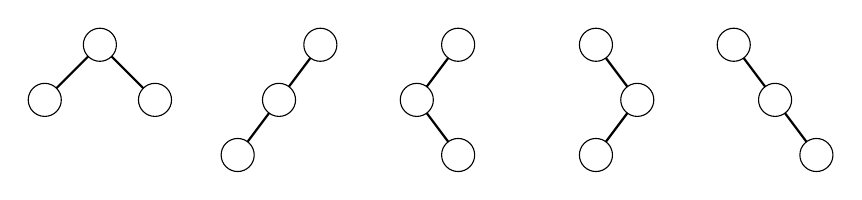
\begin{tikzpicture}[scale=0.7]
\path[draw,thick,-] (0,0) -- (-1,-1);
\path[draw,thick,-] (0,0) -- (1,-1);
\draw[fill=white] (0,0) circle (0.3);
\draw[fill=white] (-1,-1) circle (0.3);
\draw[fill=white] (1,-1) circle (0.3);

\path[draw,thick,-] (4,0) -- (4-0.75,-1) -- (4-1.5,-2);
\draw[fill=white] (4,0) circle (0.3);
\draw[fill=white] (4-0.75,-1) circle (0.3);
\draw[fill=white] (4-1.5,-2) circle (0.3);

\path[draw,thick,-] (6.5,0) -- (6.5-0.75,-1) -- (6.5-0,-2);
\draw[fill=white] (6.5,0) circle (0.3);
\draw[fill=white] (6.5-0.75,-1) circle (0.3);
\draw[fill=white] (6.5-0,-2) circle (0.3);

\path[draw,thick,-] (9,0) -- (9+0.75,-1) -- (9-0,-2);
\draw[fill=white] (9,0) circle (0.3);
\draw[fill=white] (9+0.75,-1) circle (0.3);
\draw[fill=white] (9-0,-2) circle (0.3);

\path[draw,thick,-] (11.5,0) -- (11.5+0.75,-1) -- (11.5+1.5,-2);
\draw[fill=white] (11.5,0) circle (0.3);
\draw[fill=white] (11.5+0.75,-1) circle (0.3);
\draw[fill=white] (11.5+1.5,-2) circle (0.3);
\end{tikzpicture}
\end{center}
e as árvores enraizadas são:
\begin{center}
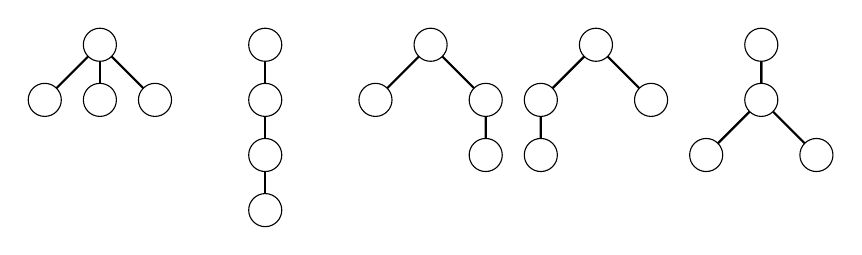
\begin{tikzpicture}[scale=0.7]
\path[draw,thick,-] (0,0) -- (-1,-1);
\path[draw,thick,-] (0,0) -- (0,-1);
\path[draw,thick,-] (0,0) -- (1,-1);
\draw[fill=white] (0,0) circle (0.3);
\draw[fill=white] (-1,-1) circle (0.3);
\draw[fill=white] (0,-1) circle (0.3);
\draw[fill=white] (1,-1) circle (0.3);

\path[draw,thick,-] (3,0) -- (3,-1) -- (3,-2) -- (3,-3);
\draw[fill=white] (3,0) circle (0.3);
\draw[fill=white] (3,-1) circle (0.3);
\draw[fill=white] (3,-2) circle (0.3);
\draw[fill=white] (3,-3) circle (0.3);

\path[draw,thick,-] (6+0,0) -- (6-1,-1);
\path[draw,thick,-] (6+0,0) -- (6+1,-1) -- (6+1,-2);
\draw[fill=white] (6+0,0) circle (0.3);
\draw[fill=white] (6-1,-1) circle (0.3);
\draw[fill=white] (6+1,-1) circle (0.3);
\draw[fill=white] (6+1,-2) circle (0.3);

\path[draw,thick,-] (9+0,0) -- (9+1,-1);
\path[draw,thick,-] (9+0,0) -- (9-1,-1) -- (9-1,-2);
\draw[fill=white] (9+0,0) circle (0.3);
\draw[fill=white] (9+1,-1) circle (0.3);
\draw[fill=white] (9-1,-1) circle (0.3);
\draw[fill=white] (9-1,-2) circle (0.3);

\path[draw,thick,-] (12+0,0) -- (12+0,-1) -- (12-1,-2);
\path[draw,thick,-] (12+0,0) -- (12+0,-1) -- (12+1,-2);
\draw[fill=white] (12+0,0) circle (0.3);
\draw[fill=white] (12+0,-1) circle (0.3);
\draw[fill=white] (12-1,-2) circle (0.3);
\draw[fill=white] (12+1,-2) circle (0.3);

\end{tikzpicture}
\end{center}

\section{Inclusão-Exclusão}

\index{inclução-exclusão}

A \key{inclusão-exclusão} é uma técnica
que pode ser usada para contar o tamanho
de uma união de conjuntos quando os tamanhos das
interseções são conhecidos e vice-versa.
Um exemplo simples da técnica é a fórmula
\[ |A \cup B| = |A| + |B| - |A \cap B|,\]
onde $A$ e $B$ são conjuntos e $|X|$
denota o tamanho de $X$.
A fórmula pode ser ilustrada da seguinte forma:

\begin{center}
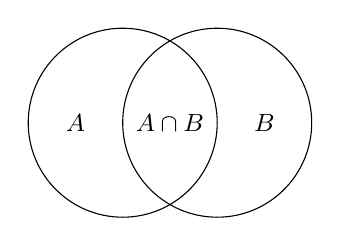
\begin{tikzpicture}[scale=0.8]

\draw (0,0) circle (1.5);
\draw (1.5,0) circle (1.5);

\node at (-0.75,0) {\small $A$};
\node at (2.25,0) {\small $B$};
\node at (0.75,0) {\small $A \cap B$};

\end{tikzpicture}
\end{center}

Nosso objetivo é calcular
o tamanho da união $A \cup B$,
que corresponde à área da região
que pertence a pelo menos um círculo.
A imagem mostra que podemos calcular
a área de $A \cup B$ primeiro somando as
áreas de $A$ e $B$ e, em seguida, subtraindo
a área de $A \cap B$.

A mesma ideia pode ser aplicada quando o número
de conjuntos é maior.
Quando há três conjuntos, a fórmula de inclusão-exclusão é
\[ |A \cup B \cup C| = |A| + |B| + |C| - |A \cap B|  - |A \cap C|  - |B \cap C| + |A \cap B \cap C| \]
e a imagem correspondente é

\begin{center}
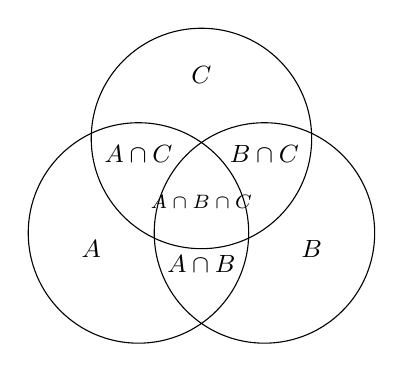
\begin{tikzpicture}[scale=0.8]

\draw (0,0) circle (1.75);
\draw (2,0) circle (1.75);
\draw (1,1.5) circle (1.75);

\node at (-0.75,-0.25) {\small $A$};
\node at (2.75,-0.25) {\small $B$};
\node at (1,2.5) {\small $C$};
\node at (1,-0.5) {\small $A \cap B$};
\node at (0,1.25) {\small $A \cap C$};
\node at (2,1.25) {\small $B \cap C$};
\node at (1,0.5) {\scriptsize $A \cap B \cap C$};

\end{tikzpicture}
\end{center}

No caso geral, o tamanho da
união $X_1 \cup X_2 \cup \cdots \cup X_n$
pode ser calculado percorrendo todas as
interseções possíveis que contenham alguns dos conjuntos $X_1,X_2,\ldots,X_n$.
Se a interseção contiver um número ímpar de conjuntos,
seu tamanho é adicionado à resposta
e, caso contrário, seu tamanho é subtraído da resposta.

Observe que existem fórmulas semelhantes
para calcular
o tamanho de uma interseção a partir dos tamanhos das
uniões. Por exemplo,
\[ |A \cap B| = |A| + |B| - |A \cup B|\]
e
\[ |A \cap B \cap C| = |A| + |B| + |C| - |A \cup B|  - |A \cup C|  - |B \cup C| + |A \cup B \cup C| .\]

\subsubsection{Desarranjos}

\index{desarranjo}

Como exemplo, vamos contar o número de \key{desarranjos}
dos elementos ${1,2,\ldots,n}$, isto é, permutações
nas quais nenhum elemento permanece em seu lugar original.
Por exemplo, quando $n=3$, existem
dois desarranjos: $(2,3,1)$ e $(3,1,2)$.

Uma abordagem para resolver o problema é usar
a inclusão-exclusão.
Seja $X_k$ o conjunto de permutações
que contêm o elemento $k$ na posição $k$.
Por exemplo, quando $n=3$, os conjuntos são os seguintes:
\[
\begin{array}{lcl}
X_1 & = & \{(1,2,3),(1,3,2)\} \\
X_2 & = & \{(1,2,3),(3,2,1)\} \\
X_3 & = & \{(1,2,3),(2,1,3)\} \\
\end{array}
\]
Usando esses conjuntos, o número de desarranjos é igual a
\[ n! - |X_1 \cup X_2 \cup \cdots \cup X_n|, \]
então, basta calcular o tamanho da união.
Usando inclusão-exclusão, isso se reduz a
calcular tamanhos de interseções, o que pode ser
feito de forma eficiente.
Por exemplo, quando $n=3$, o tamanho de
$|X_1 \cup X_2 \cup X_3|$ é
\[
\begin{array}{lcl}
 & & |X_1| + |X_2| + |X_3| - |X_1 \cap X_2|  - |X_1 \cap X_3|  - |X_2 \cap X_3| + |X_1 \cap X_2 \cap X_3| \\
 & = & 2+2+2-1-1-1+1 \\
 & = & 4, \\
\end{array}
\]
então, o número de soluções é $3!-4=2$.

Verifica-se que o problema também pode ser resolvido
sem usar inclusão-exclusão.
Seja $f(n)$ o número de desarranjos
para $\{1,2,\ldots,n\}$. Podemos usar a seguinte
fórmula recursiva:

\begin{equation*}
    f(n) = \begin{cases}
               0               & n = 1\\
               1               & n = 2\\
               (n-1)(f(n-2) + f(n-1)) & n>2 \\
           \end{cases}
\end{equation*}

A fórmula pode ser derivada considerando
as possibilidades de como o elemento 1 muda
no desarranjo.
Existem $n-1$ maneiras de escolher um elemento $x$
que substitui o elemento 1.
Em cada escolha, existem duas opções:

\textit{Opção 1:} Também substituímos o elemento $x$
pelo elemento 1.
Depois disso, a tarefa restante é construir
um desarranjo de $n-2$ elementos.

\textit{Opção 2:} Substituímos o elemento $x$
por algum outro elemento diferente de 1.
Agora temos que construir um desarranjo
de $n-1$ elementos, porque não podemos substituir
o elemento $x$ pelo elemento $1$, e todos os outros
elementos devem ser alterados.

\section{Lema de Burnside}

\index{lema de Burnside}

O \key{Lema de Burnside}
%\footnoteNa verdade, Burnside não descobriu este lema; ele apenas o mencionou em seu livro \cite{bur97}.}
pode ser usado para contar
o número de combinações, de modo que
apenas um representante seja contado
para cada grupo de combinações simétricas.
O Lema de Burnside afirma que o número de
combinações é
\[\sum_{k=1}^n \frac{c(k)}{n},\]
onde existem $n$ maneiras de mudar a
posição de uma combinação,
e existem $c(k)$ combinações que
permanecem inalteradas quando a $k$-ésima maneira é aplicada.

Como exemplo, vamos calcular o número de
colares de $n$ pérolas,
onde cada pérola tem $m$ cores possíveis.
Dois colares são simétricos se forem
semelhantes após girá-los.
Por exemplo, o colar
\begin{center}
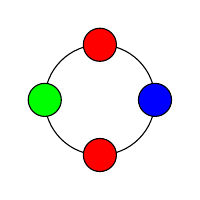
\begin{tikzpicture}[scale=0.7]
\draw[fill=white] (0,0) circle (1);
\draw[fill=red] (0,1) circle (0.3);
\draw[fill=blue] (1,0) circle (0.3);
\draw[fill=red] (0,-1) circle (0.3);
\draw[fill=green] (-1,0) circle (0.3);
\end{tikzpicture}
\end{center}
tem os seguintes colares simétricos:
\begin{center}
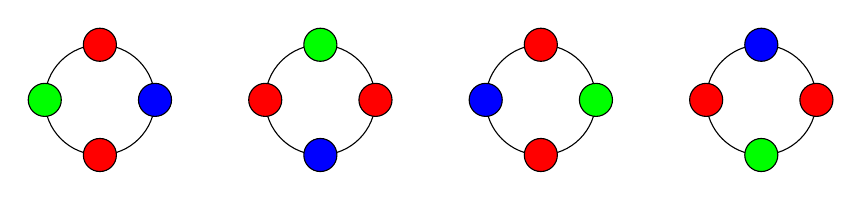
\begin{tikzpicture}[scale=0.7]
\draw[fill=white] (0,0) circle (1);
\draw[fill=red] (0,1) circle (0.3);
\draw[fill=blue] (1,0) circle (0.3);
\draw[fill=red] (0,-1) circle (0.3);
\draw[fill=green] (-1,0) circle (0.3);

\draw[fill=white] (4,0) circle (1);
\draw[fill=green] (4+0,1) circle (0.3);
\draw[fill=red] (4+1,0) circle (0.3);
\draw[fill=blue] (4+0,-1) circle (0.3);
\draw[fill=red] (4+-1,0) circle (0.3);

\draw[fill=white] (8,0) circle (1);
\draw[fill=red] (8+0,1) circle (0.3);
\draw[fill=green] (8+1,0) circle (0.3);
\draw[fill=red] (8+0,-1) circle (0.3);
\draw[fill=blue] (8+-1,0) circle (0.3);

\draw[fill=white] (12,0) circle (1);
\draw[fill=blue] (12+0,1) circle (0.3);
\draw[fill=red] (12+1,0) circle (0.3);
\draw[fill=green] (12+0,-1) circle (0.3);
\draw[fill=red] (12+-1,0) circle (0.3);
\end{tikzpicture}
\end{center}
Existem $n$ maneiras de mudar a posição
de um colar,
pois podemos girá-lo
$0,1,\ldots,n-1$ passos no sentido horário.
Se o número de passos for 0,
todos os $m^n$ colares permanecem iguais,
e, se o número de passos for 1,
apenas os $m$ colares em que cada
pérola tem a mesma cor permanecem iguais.

De forma mais geral, quando o número de passos é $k$,
um total de
\[m^{\textrm{gcd}(k,n)}\]
colares permanecem iguais,
onde $\textrm{gcd}(k,n)$ é o maior divisor comum
de $k$ e $n$.
A razão para isso é que blocos
de pérolas de tamanho $\textrm{gcd}(k,n)$
serão trocados entre si.
Assim, de acordo com o Lema de Burnside,
o número de colares é
\[\sum_{i=0}^{n-1} \frac{m^{\textrm{gcd}(i,n)}}{n}. \]
Por exemplo, o número de colares de comprimento 4
com 3 cores é
\[\frac{3^4+3+3^2+3}{4} = 24. \]

\section{Fórmula de Cayley}

\index{fórmula de Cayley}

A \key{Fórmula de Cayley}
% \footnote{Embora a fórmula tenha o nome de A. Cayley,
% que a estudou em 1889, ela foi descoberta anteriormente por C. W. Borchardt em 1860.}
afirma que 
existem $n^{n-2}$ árvores rotuladas 
que contêm $n$ vértices. 
Os vértices são rotulados como $1,2,\ldots,n$,
e duas árvores são diferentes
se sua estrutura ou
rotulagem for diferente. 

\begin{samepage}
Por exemplo, quando $n=4$, o número de árvores
rotuladas é $4^{4-2}=16$:

\begin{center}
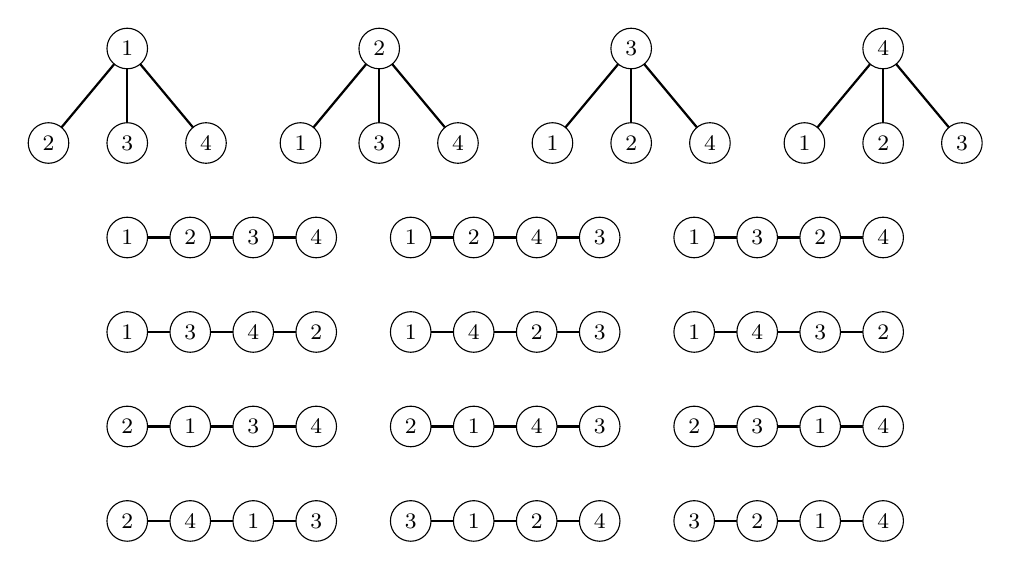
\begin{tikzpicture}[scale=0.8]
\footnotesize

\newcommand\puua[6]{
\path[draw,thick,-] (#1,#2) -- (#1-1.25,#2-1.5);
\path[draw,thick,-] (#1,#2) -- (#1,#2-1.5);
\path[draw,thick,-] (#1,#2) -- (#1+1.25,#2-1.5);
\node[draw, circle, fill=white] at (#1,#2) {#3};
\node[draw, circle, fill=white] at (#1-1.25,#2-1.5) {#4};
\node[draw, circle, fill=white] at (#1,#2-1.5) {#5};
\node[draw, circle, fill=white] at (#1+1.25,#2-1.5) {#6};
}
\newcommand\puub[6]{
\path[draw,thick,-] (#1,#2) -- (#1+1,#2);
\path[draw,thick,-] (#1+1,#2) -- (#1+2,#2);
\path[draw,thick,-] (#1+2,#2) -- (#1+3,#2);
\node[draw, circle, fill=white] at (#1,#2) {#3};
\node[draw, circle, fill=white] at (#1+1,#2) {#4};
\node[draw, circle, fill=white] at (#1+2,#2) {#5};
\node[draw, circle, fill=white] at (#1+3,#2) {#6};
}

\puua{0}{0}{1}{2}{3}{4}
\puua{4}{0}{2}{1}{3}{4}
\puua{8}{0}{3}{1}{2}{4}
\puua{12}{0}{4}{1}{2}{3}

\puub{0}{-3}{1}{2}{3}{4}
\puub{4.5}{-3}{1}{2}{4}{3}
\puub{9}{-3}{1}{3}{2}{4}
\puub{0}{-4.5}{1}{3}{4}{2}
\puub{4.5}{-4.5}{1}{4}{2}{3}
\puub{9}{-4.5}{1}{4}{3}{2}
\puub{0}{-6}{2}{1}{3}{4}
\puub{4.5}{-6}{2}{1}{4}{3}
\puub{9}{-6}{2}{3}{1}{4}
\puub{0}{-7.5}{2}{4}{1}{3}
\puub{4.5}{-7.5}{3}{1}{2}{4}
\puub{9}{-7.5}{3}{2}{1}{4}
\end{tikzpicture}
\end{center}
\end{samepage}

A seguir, veremos como a Fórmula de Cayley pode
ser derivada usando os códigos de Prüfer.

\subsubsection{Código de Prüfer}

\index{Código de Prüfer}

Um \key{Código de Prüfer}
%\footnote{Em 1918, H. Prüfer provou o teorema de Cayley usando códigos de Prüfer \cite{pru18}.}
é uma sequência de
$n-2$ números que descreve uma árvore rotulada.
O código é construído seguindo um processo
que remove $n-2$ folhas da árvore.
A cada passo, a folha com o menor rótulo é removida,
e o rótulo de seu único vizinho é adicionado ao código.

Por exemplo, vamos calcular o Código de Prüfer
do seguinte grafo:
\begin{center}
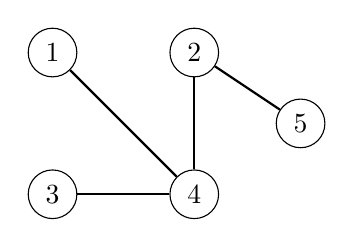
\begin{tikzpicture}[scale=0.9]
\node[draw, circle] (1) at (2,3) {$1$};
\node[draw, circle] (2) at (4,3) {$2$};
\node[draw, circle] (3) at (2,1) {$3$};
\node[draw, circle] (4) at (4,1) {$4$};
\node[draw, circle] (5) at (5.5,2) {$5$};

\path[draw,thick,-] (1) -- (4);
\path[draw,thick,-] (3) -- (4);
\path[draw,thick,-] (2) -- (4);
\path[draw,thick,-] (2) -- (5);
\end{tikzpicture}
\end{center}

Primeiro, removemos o vértice 1 e adicionamos o vértice 4 ao código:
\begin{center}
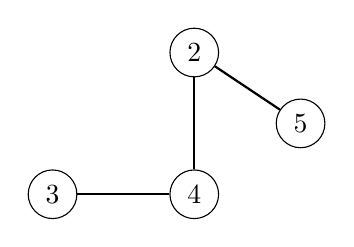
\begin{tikzpicture}[scale=0.9]
%\node[draw, circle] (1) at (2,3) {$1$};
\node[draw, circle] (2) at (4,3) {$2$};
\node[draw, circle] (3) at (2,1) {$3$};
\node[draw, circle] (4) at (4,1) {$4$};
\node[draw, circle] (5) at (5.5,2) {$5$};

%\path[draw,thick,-] (1) -- (4);
\path[draw,thick,-] (3) -- (4);
\path[draw,thick,-] (2) -- (4);
\path[draw,thick,-] (2) -- (5);
\end{tikzpicture}
\end{center}

Em seguida, removemos o vértice 3 e adicionamos o vértice 4 ao código:
\begin{center}
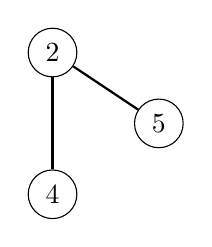
\begin{tikzpicture}[scale=0.9]
%\node[draw, circle] (1) at (2,3) {$1$};
\node[draw, circle] (2) at (4,3) {$2$};
%\node[draw, circle] (3) at (2,1) {$3$};
\node[draw, circle] (4) at (4,1) {$4$};
\node[draw, circle] (5) at (5.5,2) {$5$};

%\path[draw,thick,-] (1) -- (4);
%\path[draw,thick,-] (3) -- (4);
\path[draw,thick,-] (2) -- (4);
\path[draw,thick,-] (2) -- (5);
\end{tikzpicture}
\end{center}

Finalmente, removemos o vértice 4 e adicionamos o vértice 2 ao código:
\begin{center}
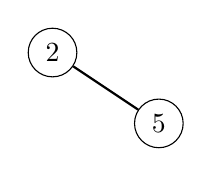
\begin{tikzpicture}[scale=0.9]
%\node[draw, circle] (1) at (2,3) {$1$};
\node[draw, circle] (2) at (4,3) {$2$};
%\node[draw, circle] (3) at (2,1) {$3$};
%\node[draw, circle] (4) at (4,1) {$4$};
\node[draw, circle] (5) at (5.5,2) {$5$};

%\path[draw,thick,-] (1) -- (4);
%\path[draw,thick,-] (3) -- (4);
%\path[draw,thick,-] (2) -- (4);
\path[draw,thick,-] (2) -- (5);
\end{tikzpicture}
\end{center}

Assim, o Código de Prüfer do grafo é $[4,4,2]$.

Podemos construir um Código de Prüfer para qualquer árvore e, mais importante,
a árvore original pode ser reconstruída
a partir de um Código de Prüfer.
Portanto, o número de árvores rotuladas
de $n$ vértices é igual a
$n^{n-2}$, o número de Códigos de Prüfer
de tamanho $n$.
